\question[10] Analiza la sucesión que se presenta en la Figura \ref{fig:sucesion_cuadros02}.


\begin{figure}[H]
    \centering
    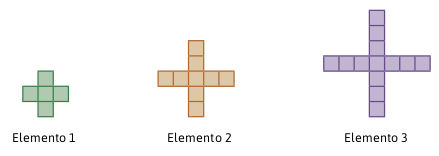
\includegraphics[width=.5\linewidth]{../images/sucesion_cuadros02}
    \caption{}
    \label{fig:sucesion_cuadros02}
\end{figure}
% \begin{multicols}{2}
\begin{parts}
    \part Completa la Tabla \ref{tab:3.7}

    \begin{table}[H]
        \centering
        \caption{}
        \label{tab:3.7}
        \begin{tabular}{r|c|c|c|c|c|c|c|c|}
            \cline{2-9}
            Posición de la figura & 1                   & 2                    & 3                    & 4                    & 5                    & 6                    & 7                    & 8                    \\ \hline
            Número de cuadrados   & \ifprintanswers5\fi & \ifprintanswers9 \fi & \ifprintanswers13\fi & \ifprintanswers17\fi & \ifprintanswers21\fi & \ifprintanswers29\fi & \ifprintanswers37\fi & \ifprintanswers61\fi \\ \cline{2-9}
        \end{tabular}
    \end{table}

    \part Escribe una regla para la sucesión.

    \begin{solutionbox}{1.5cm}
    \end{solutionbox}

    \part Reúnete en equipo y comparen sus resultados. ¿Obtuvieron una fórmula igual o equivalente? En caso necesario corrijan y argumenten por qué.

    \begin{solutionbox}{2cm}
    \end{solutionbox}
\end{parts}
% \end{multicols}
